\iffalse
\documentclass[journal,12pt,twocolumn]{IEEEtran}
\usepackage{cite}
\usepackage{amsmath,amssymb,amsfonts,amsthm}
\usepackage{algorithmic}
\usepackage{graphicx}
\usepackage{textcomp}
\usepackage{xcolor}
\usepackage{txfonts}
\usepackage{listings}
\usepackage{enumitem}
\usepackage{mathtools}
\usepackage{gensymb}
\usepackage{comment}
\usepackage[breaklinks=true]{hyperref}
\usepackage{tkz-euclide}
\usepackage{braket}
\def\inputGnumericTable{}
\usepackage[latin1]{inputenc}
\usepackage{color}
\usepackage{array}
\usepackage{longtable}
\usepackage{calc}
\usepackage{multirow}
\usepackage{hhline}
\usepackage{ifthen}
\usepackage{lscape}
\usepackage{gvv} 

\newtheorem{theorem}{Theorem}[section]
\newtheorem{problem}{Problem}
\newtheorem{proposition}{Proposition}[section]
\newtheorem{lemma}{Lemma}[section]
\newtheorem{corollary}[theorem]{Corollary}
\newtheorem{example}{Example}[section]
\newtheorem{definition}[problem]{Definition}
\newcommand{\BEQA}{\begin{eqnarray}}
\newcommand{\EEQA}{\end{eqnarray}}
\newcommand{\define}{\stackrel{\triangle}{=}}
\theoremstyle{remark}
\newtheorem{rem}{Remark}

\begin{document}

\bibliographystyle{IEEEtran}
\vspace{3cm}

\title{GATE 2022 BM-42}
\author{EE23BTECH11201 - Abburi Tanusha$^{*}$% <-this % stops a space
}
\maketitle
\newpage
\bigskip

\renewcommand{\thefigure}{\theenumi}
\renewcommand{\thetable}{\theenumi}

\vspace{3cm}

\maketitle
\textbf{Question:} 
If 
\begin{align}
 g(t) &= \frac{df(t)}{dt} \\
 F(s) &= \frac{1+s}{s^2+12s+32} 
\end{align} 
where $F(s)$ is the Laplace transform of the function $f(t)$, then what is the value of $g(t)$ at $t=0$ ?\\
\hfill(GATE BM 2022)\\
\textbf{Solution:} 
\fi
\begin{table}[h!]
\centering
\resizebox{6cm}{!}{

\begin{tabular}{|c|c|c|}
\hline
\textbf{Value} & \textbf{Parameter} & \textbf{Description} \\
\hline
$g(t)$ & $\frac{df(t)}{dt}$ & Derivative of $f(t)$ with respect to $t$ \\
\hline
$F(s)$ & $\frac{1+s}{s^2+12s+32}$ & Laplace transform of the function $f(t)$ \\
\hline

\end{tabular}



}
\caption{Given Parameters}
\label{tab:tanu_tabel}
\end{table}

Using Initial value Theorem 
\begin{align}
    f(0) &= \lim_{s \to \infty} sF(s) \\
         &= \lim_{s \to \infty} \frac{s(s+1)}{s^2 + 12s + 32} \\
         &= 1 \\
    G(s) &= sF(s) - f(0) \\
         &= \frac{s(s+1)}{s^2 + 12s + 32} - 1 \\
         &= \frac{s^2 + s - (s^2 + 12s + 32)}{s^2 + 12s + 32} \\
         G(s) &= \frac{-11s - 32}{s^2 + 12s + 32} 
\end{align}
Using Partial fraction decomposition 
\begin{align}
      G(s)   &= \frac{A}{s+4} + \frac{B}{s+8}  \\
    -11s - 32 &= A(s+8) + B(s+4) \\
    -11s - 32 &= (A + B)s + (8A + 4B)
\end{align}
Equating coefficients:
\begin{align}
     -11 &= A + B \\
    -32 &= 8A + 4B
\end{align}
By solving these equations , we get 
\begin{align}
    A &= 3 \\
    B &= -14 \\
    G(s) &=\frac{3}{s+4} - \frac{14}{s+8} ; \quad Re(s) > -4
\end{align}
Inverse Laplace transform of $G(s)$ 
\begin{align}
g(t) &=\mathcal{L}^{-1}\brak{\frac{3}{s+4}} -\mathcal{L}^{-1}\brak{\frac{14}{s+8}} \\
   &= 3e^{-4t} - 14e^{-8t} \\
g(0) &= 3e^{-4 \cdot 0} - 14e^{-8 \cdot 0} \\
         &= 3 - 14 \\
         &= -11
\end{align}
Verifying g(0) by Initial value theorem
\begin{align}
    g(0) &= \lim_{s \to \infty} sG(s) \\
         &= \lim_{s \to \infty} s \cdot \frac{-11s - 32}{s^2 + 12s + 32} \\
         &= \lim_{s \to \infty} \frac{-11 - \frac{32}{s}}{1 + \frac{12}{s} + \frac{32}{s^2}} \\
         &= \lim_{s \to \infty} \frac{-11}{1} \\
         &= -11
\end{align}
The value of $g(t)$ at $t=0$ is $-11$.
\begin{figure}[h!]
\centering
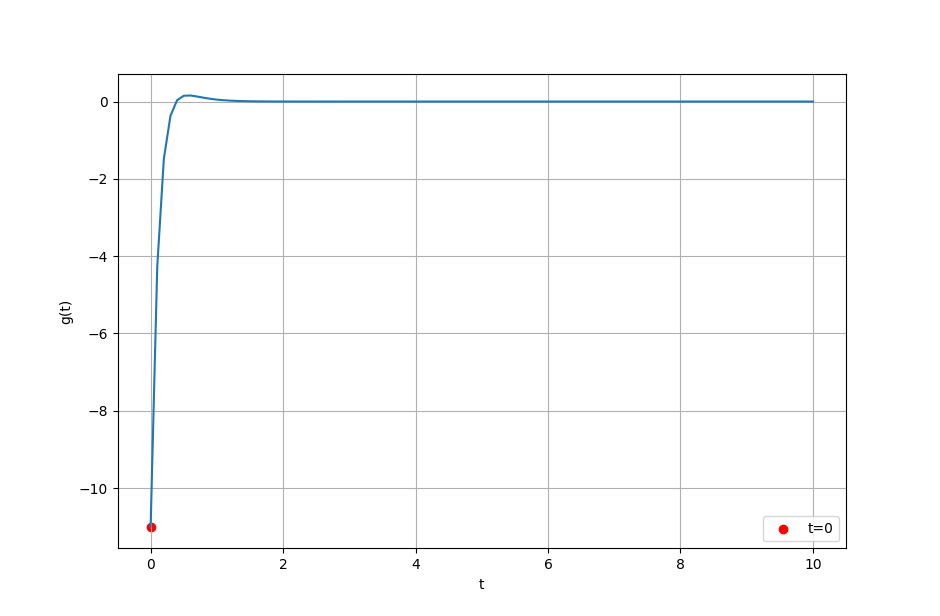
\includegraphics[width=\columnwidth]{2022/BM/42/figs/stem_plot.png}
\caption{Plot $g(t)$ vs $t$ }
\label{fig:tansh_plott}
\end{figure}
%\end{document}
